\documentclass[12pt]{article}

\usepackage{sbc-template}
\usepackage[utf8]{inputenc}
\usepackage{graphicx,url}
\usepackage[brazil]{babel}   
\usepackage[latin1]{inputenc}  
\sloppy

\title{Estrutura conceitual do Modelo para Agentes Normativos}

\begin{document} 

\section{Objetivo}

O modelo proposto tem como por finalidade representar atividades onde um grupo de pessoas  devem atuar de forma colaborativa com o propósito de resolver um problema. Esse problema pode ser dividido em etapas menores conhecidas como objetivos. Essas pessoas podem se relacionar entre sí, podem se relacionar com os artefatos presentes no meio 
onde elas atuam. Os artefatos também possuem a capacidade de se relacionar. Cada objetivo é concluído apenas se  um ou mais relacionamentos forem realizados. A conclusão do objetivo também é função de certos agentes e artefatos que devem ser presentes. 

Outra finalidade do modelo consiste em representar condições que devem ser mantidas ao longo da atividade, se essas condições forem desfeitas - a atividade deve ser encerrada de imediato, caso contrário as pessoas envolvidas nesta manutenção estarão submetidas a risco de morte. Dentro desta abordagem, alguém designado para cumprir com alguma atividade pode cometer erros. Esse modelo tem como por finalidade lidar com os seguintes tipos de erro: não executar algum ação quando essa ação deve ser executada, executar uma ação quando ela não deve ser executada, executar uma ação quando não há condições apropriadas para isso, manipular artefatos de maneira inapropriada ou inadvertida e escolher os artefatos inapropriados para cumprir com uma determinada atividade.

O modelo deve ser capaz de representar as consequências desses erros. Esse modelo está preocupado em representar dois tipos de consequências, essas são: 1 - imediatas que acontece sobre o indivíduo errante, 2 - a consequência manifesta em outro objetivo sobre o mesmo ou outro indivíduo pertencente ao grupo. Essas consequências são efeitos físicos negativos que alguém vêem a sofrer. A intensidade dessas consequências variam desde uma leve lesão a morte.

Outro aspecto deste modelo consiste representar objetivos cujo sucesso advem de certa característica aleatória presente na natureza da atividade. Essa característica aleatória consiste em um evento que possuem uma certa possibilidade de acontecer. Se esse evento acontecer, alguém sofre consequências ruins por conta disto. O modelo deve considerar relações entre erros onde as consequências se manifestam de forma indireta com eventos aleatórios.         

\section{Exemplo - Estudo de Caso}

Sete profissionais de linha viva (profissionais que realizam manutenção em equipamentos elétricos energizados) são designados com o propósito de realizar a substituição de um isolador de pedestal. Os papéis desses desses profissionais são; 1 supervisor, 1 observador e 5 executores. A manutenção de ve ser executada apenas sobre as seguintes condições: céu ensolarado e umidade relativa do ar menor que 70 porcento. Todos os profissionais devem possuir os EPIS necessários: capacete, óculos de sol, roupa isolante e anti-chamas, luvas isolantes e botas isolantes. Os profissionais que entrarão no potencial deverão estar vestidos de roupa condutiva e cabo guarda. As ferramentas necessárias para resolver esse problema são: bastão garra de diametro 64 x 3600 mm, sela de diametro 65 , colar, corda de fibra sintética, carretilha, chave com catraca, bastão universal, soquete adequado, locador de pino, bastão com soquete multiangular. A substitução do isolador de pedestal pode ser escrita nos seguintes subobjetivos: 


\begin{enumerate}
	\item Limpar, secar e testar corda.
	\item Instalar Bastão Garra na estrutura com o pedestal a ser substituído.
	\item Instalar sela com colar na estrutura
	\item Amarrar o bastão na parte superior da estrutura com a corda.
	\item Amarrar o olhal do bastão ao cavalo da sela atras de uma corda.
	\item Instalar um segundo conjunto bastão e sela no lado oposto da estrutura.
	\item Enforcar um estropo de Náilon no corpo do isolador.
	\item Colocar a extremidade do estropo no gancho da corda de serviço.
	\item Afrouxar os parafusos do conector que prendem a barra ao isolador.
	\item Terminar de retirar os parafusos com o bastão com o soquete multiangular.
	\item Elevar a barra através da corda que une a sela ao bastão.
	\item Apertar o colar através da porca borboleta.
	\item Segurar firmemente a corda de serviço.
	\item Sacar parafusos da base da coluna.
	\item Baixar o isolador ao solo
	\item Içar o Isolador
	\item Colocar Parafusos na base da coluna.
	\item Baixaer a barra para que a mesma apóie no novo isolador.
	\item Colocar os parafusos do conector que prende a barra ao novo isolador. 
	\item Retirar Equipamentos
\end{enumerate}

\section{Modelo}

\subsection{Definição dos Conjuntos}

\begin{enumerate}
	\item $Entity = \{e_1, ..., e_n\}$ - conjunto de todas as Entidades.  
	\item $Agent = \{ag_1, ..., ag_n\}$ - conjunto dos Agentes.
	\item $Artefact = \{at_1, ..., at_n\}$ - conjunto dos Artefatos.
	\item $EntityGoal = eg = \{e_n,...,e_m\}$ - conjunto das Entidades que devem estar presentes para concluir um determinado objetivo $g_i$.
	\item $Relation = \{r_1, ..., r_n\}$ - conjunto dos Relacionamentos.	
	\item $RelationGoal = rg =\{r_n, ..., r_m\}$ - conjunto dos Relacionamentos que devem estar presentes para concluir um único objetivo $g_i$.		
	\item $Role = \{\rho_1, ..., \rho_n\}$ - conjunto dos Papéis.	
	\item $Goal = \{g_1, ..., g_n\}$ - conjunto dos Objetivos.
	\item $GoalRandomic = \{gr_1,..., gr_n\}$ - conjunto dos Objetivos	Randomicos.
	\item $GoalPrerequisit = gp = \{g_n,...,g_m\}$ - conjunto de Objetivos que são pré-requisitos para alcançar um outro objetivo.
	\item $Condition = \{c_1, ..., c_n\}$ - conjunto das Condições que devem ser mantidas ao longo da execução de todos os objetivos.
	\item $ConditionToGoal = cg = \{c_n, ..., c_m\}$ - conjunto de condições que devem ser mantidas para concluir um único objetivo $g_i$.
	\item $Risk = \{risk_1, ..., risk_n\}$ - conjunto dos Riscos na ocorrência de Eventos Ruins.
	\item $Possibility = \{p_1, ..., p_n\}$ - conjunto das possibilidades de Eventos Ruins. 
	\item $Fatality = \{f_1, ..., f_n\}$ - conjunto das fatalidades que acontecem na existência de um evento ruim. 	
\end{enumerate}


\subsection{Definição das Relações Entre os Conjuntos}

\begin{enumerate}
	\item $Entity \equiv Agent \cup Artefact$
	\item $Agent$ e $Artefact$ são disjuntos.
	\item $GoalRadomic \subset Goal$
	\item $\{gp_1,...,gp_n\} \subset Goal$
	\item $\{cg_1,...,cg_n\} \subset Condition$
	\item $\{eg_1,...,eg_n\} \subset Entity$		
	\item $\{rg_1,...,rg_n\} \subset Relation$	
\end{enumerate}

\subsection{Definição dos Predicados}

\begin{enumerate}
	\item $relationHas(r_l,e_i,e_k)$ onde $i \neq j$ - Um determinado relacionamento $r_l$ é composto por uma entidade $e_i$ e $e_k$ onde $e_i$ não pode ser igual a $e_j$.	
	\item $hasRole(ag_n,\rho_m)$ - Um determinado agente $ag_n$ tem um determinado papel $\rho_m$.
	\item $hasObligation(\rho_m,g_j)$ - Quem assume o papel $\rho_m$ é obrigado a concluir o objetivo $g_j$.
	\item $hasPermission(\rho_m,g_j)$ - Quem assume o papel $\rho_m$ tem a permissão de concluir o objetivo $g_j$.
	\item $isReached(g_k)$ - O objetivo $g_k$ foi alcançado.
	\item $isPreRequisite(gp_i,g)$ - Os objetivos $g$ pertencentes ao grupo $gp_i$ devem ser concluidos para que haja condição de executar g.
	\item $hasCondition(g_i,cg_n)$ - Um objetivo do tipo $g_i$ possui certas condições $c$ que deve estar presentes e devem se manter durante toda execução deste objetivo. Essas condições $c$ devem estar conditdas em $cg_n$. 
	\item $hasEntity(g_i,eg_i)$ - Um objetivo $g_i$ tem um conjunto de entidades $eg_i$ onde todas as entidades presentes neste conjunto devem estar presentes no momento da execução desse objetivo.
	\item $hasRelation(g_i,rg_i)$ - Um objetivo $g_i$ tem um conjunto de relacionamentos $rg_i$ onde todos esses relacionamentos devem ser feito para que este objetivo seja concluído.
	\item $isPresent(cg_n)$ - Todas as condições pertencentes a $cg_n$ estão presentes.
	\item $tryReach(ag_i,g_j)$ - Um determinado agente $ag_i$ tenta alcançar o objetivo $g_j$.
	\item $violationCondition(ag_i,g_j,c_k)$ - Um determinado agente $ag_i$ comete uma violação de condição no objetivo $g_j$ sobre a condição $c_k$. 
	\item $violationNotPermission(ag_i,g_j)$ - O agente $ag_i$ comete uma violação de não permissão $g_j$ - tentativa de alcançar um objetivo mesmo sem ter permissão para isso. 
	\item $violationObligation(ag_i,g_j)$ - O agente $ag_i$ comete uma violação de obrigação $g_j$ - não executa o objetivo mesmo quando é obrigado a fazer isso e quando o objetivo está no momento certo de ser executado.
	\item $violationRelation(ag_i,g_j,r_k)$ - O agente $ag_i$ comete uma violação de Relacionamento no objetivo $g_j$ por não realizar o relacionamento $r_k$. 
	\item $violationEntity(ag_i,g_j,e_k)$ - O agente $ag_i$ comete uma violação de Entidade no objetivo $g_j$ por tentar alcançar esse objetivo sem ter a entidade $e_k$ presente.  	
	\item $hasRisk(c_k,risk_j,f_m)$ - A condição $c_k$ está associada a um risco $risk_k$ com uma certa fatalidade $f_m$. 
	\item $hasRisk(r_k,risk_j,f_m)$ - O relacionamento $r_k$ está associado a um risco $risk_k$ com uma certa fatalidade $f_m$.
	\item $hasRisk(e_k,risk_j,f_m)$ - A entidade $e_k$ está associada a um risco $risk_k$ com uma certa fatalidade $f_m$.
	\item $badEvent(ag_i,risk_j,f_m)$ - Agente $ag$ sofre as consequências do risco $risk_j$ com a fatalidade $f_m$
\end{enumerate}








\textbf{Definição 7}

\begin{equation}
	attribution(ag,\rho_{r_i})\wedge deonticRelation(\rho_{r},g_{e_i},d_{o_i}) \to obligation(ag,g_{e_i}) 
\end{equation}


\textbf{Motivo} 

Se um agente posssui atribuição de um papel e se um determinado objetivo está dentro do escopo deste papel, então esse agente possui a obrigação de alcançar este objetivo.



\textbf{Definição 8}

\begin{equation}
  attribution(ag,\rho_{r_i})\wedge deonticRelation(\rho_{r_i},g_{e_i},d_{p_i}) \to permission(ag,g_{e_i}) 
\end{equation}



\textbf{Motivo} 

Se um agente posssui atribuição de um papel e se um determinado objetivo está dentro do escopo deste papel, então esse agente possui a permissão de alcançar este objetivo.


\textbf{Definição 9}

\begin{equation}
  obligation(ag,g_{e_i}) \to permission(ag,g_{e_i}) 
\end{equation}


\textbf{Motivo} 

Toda a obrigação implica em uma permissão. 


\textbf{Definição 10}

Se para iniciar um determinado objetivo $ g_{e_j} $ é necessário completar outros objetivos, $ g_{e_i}, ... g_{e_k} $, se pelo menos um destes objetivos for falso para $ isCompleted(g_x), x = i,..,k $, então $ preCondition(g_j,(g_{i},...g_{k})) $ é falso, se não, então  $ preCondition(g_j,(g_{i},...g_{k})) $ é verdadeiro.

Sendo que existe um conjunto $ g_{preRequisit} = \{g_{i},...g_{k}\} $, então

\begin{eqnarray}
  (preCondition(g_j,g_{preRequisite}) \to preRequisit(g_j)) \wedge  \\ \neg (preCondition(g_j,g_{preRequisite}) \to \neg preRequisit(g_j))  
\end{eqnarray}

\textbf{Motivo} 

Um objetivo pode ser executado apenas se os pre-requisitos forem alcançados. 


\textbf{Definição 11}

Sendo $cm$ conjunto de condições que devem ser mantidos o tempo inteiro para que a atividade possa acontecer,
\begin{eqnarray}
    preRequisit(g_{e_i}) \wedge hasMaintainer(g_{e_i},cm_i) \wedge isOk(cm_i) \to canStart(g_{e_i}) 
\end{eqnarray}

\textbf{Motivo} 

Considerações que devem ser alcançadas e mantidas para que um determiando objetivo tenha condições de começar a ser alcançado. Essas considerações consiste em ter os seus pre-requisitos alcançados (Definição 10), e as condições temporais devem possibilitar a atividade.  



\textbf{Definição 12} 

\begin{eqnarray}
    preRequisit(g_{e_i}) \wedge hasMaintainer(g_{e_i},cm_i) \wedge \neg isOk(cm_i) \wedge  tryReach(g_{e_i},ag) \to  \\ violation(g_{e_i},ag,cm_i)    
\end{eqnarray}

\textbf{Motivo} 

Se o agente tentar executar um determinado objetivo mesmo que as condições    

\textbf{Definição 13}

Se $ attribution(ag,\rho_{r}) \wedge \neg deonticRelation(\rho_{r},g_{e_i},d_{p_i}) \wedge canStart(g_{e_i}) \wedge tryReach(g_{e_i},ag) $ é verdade, então $ violation(d_{p_i},ag) $ é verdade. Contudo, se $ attribution(ag,\rho_{r}) \wedge \neg deonticRelation(\rho_{r},g_{e},d_{p_i}) \wedge canStart(g_e) \wedge tryReach(g_{e_i},ag) $ for falso, então $ violation(d_{p_i},ag) $.

\textbf{Definição 14} 

Existe $c_r$, onde $c_r$ é um conjunto que mapeia as relações das entidades da pela relação $isRelationOf(r_j,c_{r_i})$. Cada $g_{e_i}$ possui um $c_{r_i}$ dada pela relação $hasConditionRelation(g_{e_i},c_{r_i})$. Se $ permission(ag,g_{e_i}) \wedge canStart(g_{e_i}) \wedge hasConditionRelation(g_{e_i},c_{r_i}) \wedge isRelationOf(r_j,c_{r_i}) \wedge \neg know(ag,r_j) \wedge tryReach(ag,g_{e_i})$ é verdade, então é verdade $ violation(r_j,g_{e_i},ag) $. Contudo $ violation(r_j,g_{e_i},ag) $ é falso para a condição de $ permission(ag,g_{e_i}) \wedge canStart(g_{e_i}) \wedge hasConditionRelation(g_{e_i},c_{r_i}) \wedge isRelationOf(r_j,c_{r_i}) \wedge \neg know(ag,r_j) \wedge tryReach(ag,g_{e_i})$ ser falsa.

\textbf{Definição 15}

Se $ permission(ag,g_{e_i}) \wedge canStart(g_{e_i}) \wedge hasConditionRelation(g_{e_i},c_{r_i}) \wedge isRelationOf(r_j,c_{r_i}) \wedge \neg execute(ag,r_j) \wedge tryReach(ag,g_{e_i})$ é verdade, então é verdade $ violation(r_j,g_{e_i},ag) $. Contudo $ violation(r_j,g_{e_i},ag) $ é falso para a condição de $ permission(ag,g_{e_i}) \wedge canStart(g_{e_i}) \wedge hasConditionRelation(g_{e_i},c_{r_i}) \wedge isRelationOf(r_j,c_{r_i}) \wedge \neg execute(ag,r_j) \wedge tryReach(ag,g_{e_i})$ ser falsa.

\textbf{Definição 16}

Se $ attribution(ag,\rho_{r}) \wedge deonticRelation(\rho_{r},g_{e_i},d_{o_i}) \wedge canStart(g_{e_i}) \wedge \neg tryReach(ag,g_{e_i}) $ então existe uma violação dada como $ violation(d_{o_i},ag,g_{e_i}) $. Se não $ violation(d_{o_i},ag,g_{e_i}) $ é falso.

\textbf{Definição 17} 

Existe um conjunto $ c_e $, condition entity, que mapeia as entidades necessárias $ isEntityOf(e_k,c_{e_i})$ para que um determinado objetivo possa ser alcançado. Para cada $ g_{e_{i}} $ existe uma dada relação em que $ hasConditionEntity(g_{e_i},c_{e_i}) $. Sendo assim, $ permission(ag,g_{e_i}) \wedge tryReach(ag,g_{e_i}) \wedge canStart(g_{e_i}) \wedge hasConditionEntity(g_{e_i},c_{e_i}) \wedge isEntityOf(e_k,c_{e_i}) \wedge \neg isInMomentOfGoal(e_k,g_{e_i}) \to  violation(g_{e_i},e_k,ag) $. Contudo, é verdadeiro $ \neg violation(g_{e_i},e_k,ag) $ se $ hasConditionEntity(g_{e_i},c_{e_i}) \wedge tryReach(ag,g_{e_i}) \wedge canStart(g_{e_i}) \wedge hasConditionEntity(g_{e_i},c_{e_i}) \wedge isEntityOf(e_k,c_{e_i}) \wedge \neg isInMomentOfGoal(e_k,g_{e_i}) $ é falso. A relação $isInMomentOfGoal(e_k,g_{e_i})$ indica se entidade estará disponível no momento que o agente $ag$ tenta alcançar o objetivo $g_{e_i}$.

\textbf{Definição 18} 

\begin{equation}
attribution(ag,\rho_a) \to obligation(ag,g_d)
\end{equation}

\textbf{Definição 19}

Se for verdade $ obligation(ag_i,g_d) \wedge delegate(ag_i,\rho_{r_i},ag_j) \wedge deonticRelation(\rho_{r_i},g_{e_i},d_{p}) \wedge hasConditionRelation(g_{e_i},c_{r_i}) \wedge isRelation(r_k,c_{r_i}) \wedge \neg know(ag_j,r_k) $ então ocorre uma violação em $violation(\rho_{a},g_{d},ag_{i})$. Se não,  $ \neg violation(\rho_{a},g_{d},ag_{i}) $ é verdade.

\textbf{Definição 20}

\begin{eqnarray}
violation(d_{p_i},ag) \to stopOperation \\
\neg violation(d_{p_i},ag) \to \neg stopOperation 
\end{eqnarray}

\textbf{Definição 21}

\begin{eqnarray}
violation(r_j,g_{e_i},ag) \wedge isGoalRandon(g_{e_j}) \wedge hasPossibilityBadEvent(g_{e_j},p_1) \\  
\to hasPossibilityBadEvent(g_{e_j},p_2) \wedge p_2 > p_1 \\
\neg violation(r_j,g_{e_i},ag) \wedge isGoalRandon(g_{e_j}) \wedge hasPossibilityBadEvent(g_{e_j},p_1) \\  
\to hasPossibilityBadEvent(g_{e_j},p_1) 
\end{eqnarray}

\textbf{Definição 22}

\begin{eqnarray}
violation(r_j,g_{e_i},ag) \to sanction(g_{e_i},ag,risk) \to badEvent(risk,fatality,ag,g_{e_i}) \\
\neg violation(r_j,g_{e_i},ag) \to \neg sanction(g_{e_i},ag,risk) \to \neg  badEvent(risk,fatality,ag,g_{e_i})
\end{eqnarray}


\textbf{Definição 23}

\begin{eqnarray}
hasPossibilityBadEvent(g_{e_j},p) \wedge eventBadHappens(g_{e_j}) \wedge tryReach(ag,g_{e_j}) \\ \to badEvent(risk,fatality,ag,g_{e_j}) \\ 
hasPossibilityBadEvent(g_{e_j},p) \wedge \neg eventBadHappens(g_{e_j}) \wedge tryReach(ag,g_{e_j}) \\ \to \neg badEvent(risk,fatality,ag,g_{e_j}) \\
hasPossibilityBadEvent(g_{e_j},p) \wedge  eventBadHappens(g_{e_j}) \wedge \neg tryReach(ag,g_{e_j}) \\ \to \neg badEvent(risk,fatality,ag,g_{e_j}) 
\end{eqnarray}

\textbf{Definição 24}

\begin{eqnarray}
violation(d_{o_i},ag,g_{e_i}) \to stopOperation \\
\neg violation(d_{o_i},ag,g_{e_i}) \to \neg stopOperation 
\end{eqnarray}

\textbf{Definição 25}

\begin{eqnarray}
	violation(g_{e_i},e_k,ag) \to sanction(g_{e_i},ag,risk) \to badEvent(risk,fatality,ag,g_{e_i}) \\
	\neg violation(g_{e_i},e_k,ag) \to \neg sanction(g_{e_i},ag,risk) \to \neg badEvent(risk,fatality,ag,g_{e_i})
\end{eqnarray}

\textbf{Definição 26}

\begin{eqnarray}
	violation(g_{e_i},ag,cm_i)  \to sanction(g_{e_i},ag,risk) \to badEvent(risk,fatality,ag,g_{e_i}) \\
	\neg violation(g_{e_i},e_k,ag) \to \neg sanction(g_{e_i},ag,risk) \to \neg badEvent(risk,fatality,ag,g_{e_i})
\end{eqnarray}

\textbf{Definição 27}

\begin{eqnarray}
	badEvent(risk,fatality,ag,g_{e_i}) \to stopOperation \\
	\neg badEvent(risk,fatality,ag,g_{e_i}) \to \neg stopOperation
\end{eqnarray}

\textbf{Definição 28}

Para todos os agentes que receberam uma obrigação de executar $g_{e_i}$, ao cumprir com a condição $ tryReach(g_{e_i},ag) \wedge \neg stopOperation $ então $ isCompleted(g_{e_i})$, se não, então é verdade $ failed(g_{e_i}) $

\begin{figure}
  \centering
  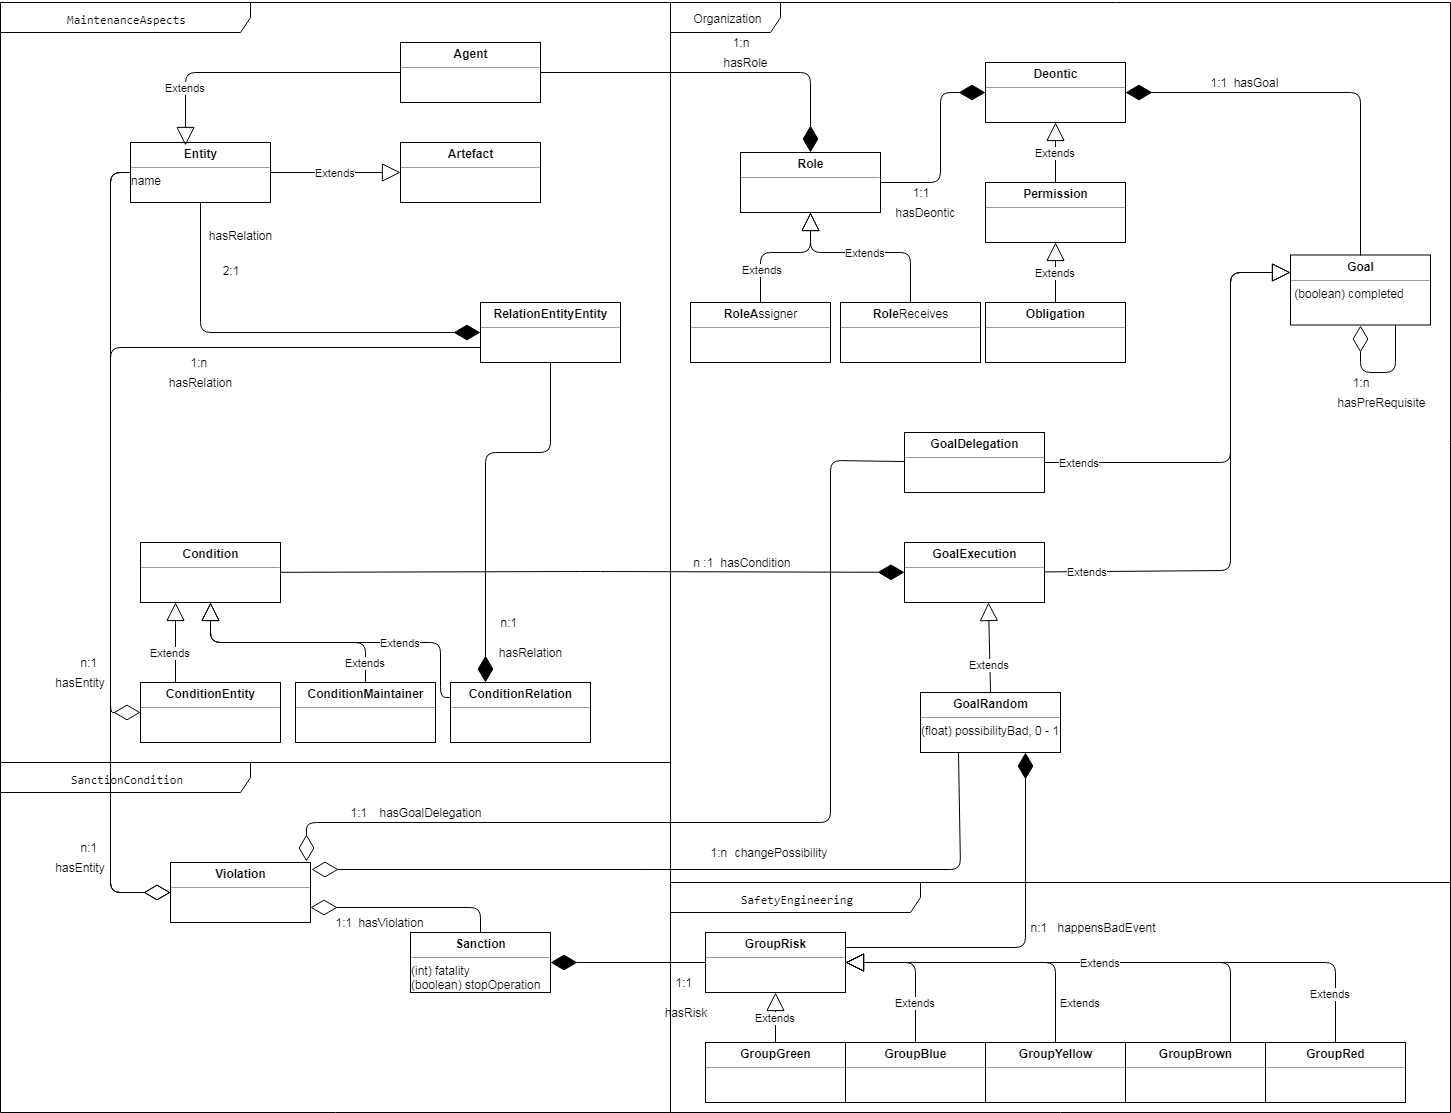
\includegraphics[width=0.8\linewidth]{umlmodel} 
\end{figure}

\end{document} 
